In this chapter we describe \demo~\cite{korsveien2014vizpub}, a tool we
propose for visualizing the performance of overlay-based Pub/Sub
Systems. We presented poster and held a live demonstration of our system
at the ACM International Conference of Distributed Event Based Systems
(DEBS), held in Mumbai in May 2014, where it was awarded the price for
best poster/demo!

\section{System Overview}

To the best of our knowledge, \demo~is the first tool of its kind. The
tool is able to visualize the execution of any given distributed pub/sub
system step by step with respect to a set of performance metrics. Each
node in the system records records relevant data at selected
\emph{reporter intervals} during system execution. Our tool is then able to pull this data to a
single site, and compute various metrics at a system-wide scale. The
collected data from each interval is then collated into a single
gexf-file, which is interpreted by Gephi, which enable replay of system
execution offline.

Our tool supports two types of visualizations visualizations, the first is a
visualization of the overlay structure, and how it evolves over time.
The second type of animation is a hop-by-hop visualization of a single
publication message dissemination, where directed edges represent the
message dissemination path. We provide examples of both types of
visualizations later in this chapter.

There are several benefits to using a tool such as \demo. It enables
researchers and developers to gain a deeper insight into the overlay
structure as well as the publication process. It also has major benefits
as an educational tool, as it provides students with an visual
representation of both the structural evolution of the system, as well
as step-by-step animations of publication message disseminations. This
is useful in order to engage students, and facilitate deeper insight
into different pub/sub systems and their dissemination schemes. Such an
insight is also useful in order to identify potential weaknesses or
deployment anomalies of a given pub/sub systems. When developing the
tool, we encountered many scenarios where \demo~demonstrated its
usefulness. For example, when experimenting with PolderCast, we could
immediately verify that tree nodes were disconnected at the RINGS layer,
as seen in Figure~\ref{fig:pold_disc}.  Using our tool, we were able to
verify that this was caused by an artefact in the input workload where
the three nodes had no overlapping interest with any other node in the
system. We were then able to verify that the nodes were connected at the
CYCLON layer. We are not aware of any other tool or framework that would
allow such easy detection and validation of system behaviour.

\begin{figure}[h]
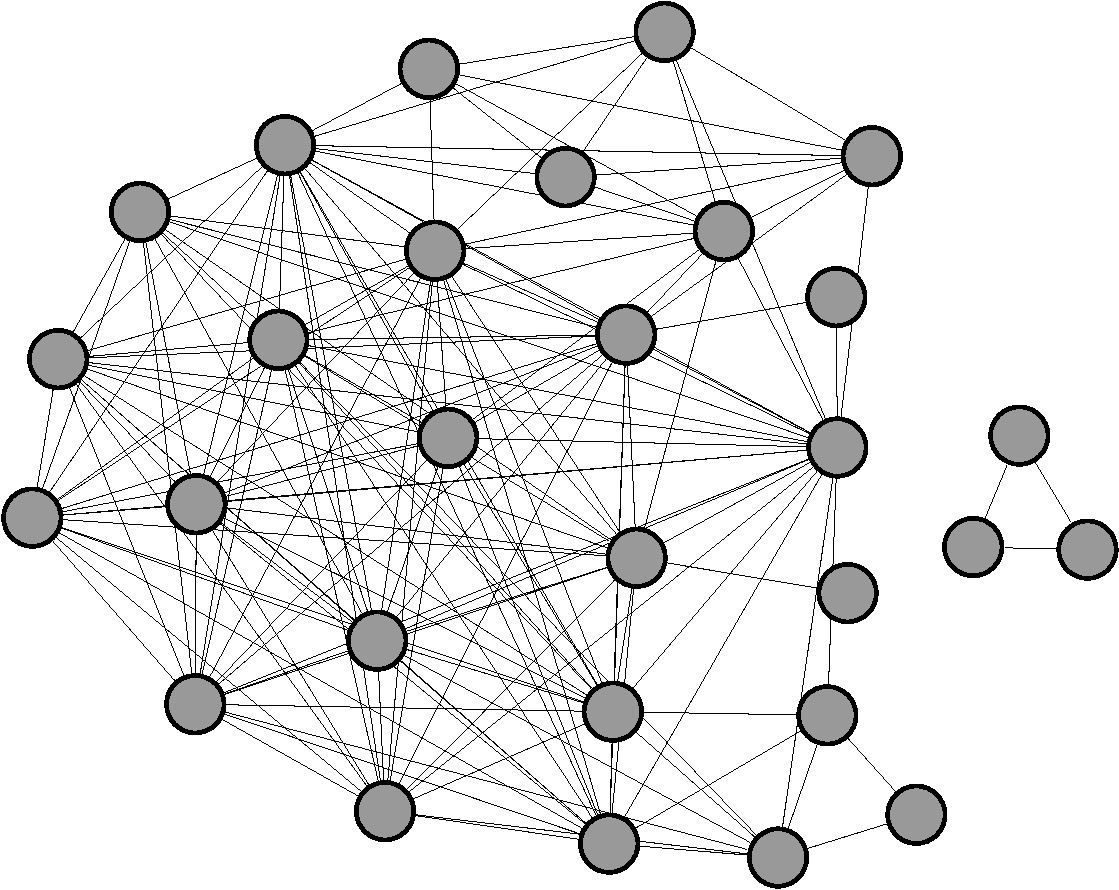
\includegraphics[width=\linewidth]{figures/disconnected-component-poldercast.pdf}
\caption{Visualization of disconnected component in the RINGS layer of PolderCast}
\label{fig:pold_disc}
\end{figure}

Another interesting use case for our tool is comparing different pub/sub systems and
protocols visually. Users may run the different systems using the same
workload, e.g.\ subscriptions and publications, and system parameters in
order to replay the execution and compare the different systems at
selected points in time. We include such comparisons in this chapter,
were we compare PolderCast and Scribe on a set of specific performance
metrics.

\section{Supported Metrics}
\label{sec:metrics}

\section{System Architecture}

\begin{figure}[h]
\centering
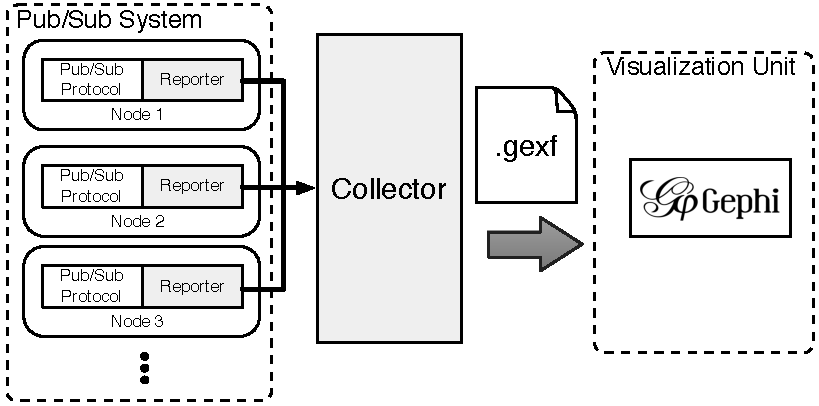
\includegraphics[width=\linewidth]{figures/arch}
\caption{Architecture diagram of \demo}
\label{fig:arch}
\end{figure}

The architecture of \demo~consists of three main components, all
depicted in Figure~\ref{fig:arch}: (1) \emph{Reporter}, (2)
\emph{Collector} and (3) \emph{Visualization Unit}.  The arrows seen in
Figure~\ref{fig:arch} depicts the flow of data in the architecture.
Each node in the executing system consists of a pub/sub protocol as well
as a ``Reporter''. The ``Reporter'' is the entity responsible for
providing the raw information required to compute various performance
metrics from the individual nodes participating in the overlay. This
information is pulled at regular intervals to a central site by the
``Collector'', which translates stores the information as a single
file in the GEXF-format. This file is then interpreted by the
``Visualization Unit'', which consists of a single machine running
the Gephi tool. The Collector is designed to perform the collection of
data while in online mode, while the computation, aggregation and
derivation of various metrics is performed in in offline mode. The
Visualization Unit always operate in offline mode, as it waits for the
final report to be collated into a GEXF-format for playback and
visualization.

The design of \demo~supports pub/sub systems that are deployed as
real distributed systems, as well as systems that are deployed in
simulation mode. This is due to the highly modular system architecture,
with strict separation of concerns, where the operation of both the
Collector and the Visualization Unit is separate from the reporting.
\demo~is designed to be a generic tool, where the only system specific
part of the architecture is the \emph{reporter interface} outlined in
Table~\ref{table:interface}. Any researcher or developer
who wants to use our framework only needs to provide an implementation
of this interface, which enables the Collector to retrieve the relevant
data from each individual node at the specified time points. These time
points are configurable, and all the information collected from the
reporter will in effect be the change of the system state from the last
time point with regards to the various performance metrics. We call
these time points \emph{reporting intervals}. The length of the intervals
is configurable, which provides the user with control over the
granularity of data collection, and thus the granularity of the
step-by-step replay of system execution performed in the Visualisation Unit. For example, if
running simulation using PeerNet, the user may determine whether or not
the reporting intervals should encompass several simulation cycles. Or,
in a real distributed pub/sub deployment scenario, the user can
determine the time delay between every reporting interval.


\subsection{Reporter}

The Reporter is responsible of providing the relevant data necessary in
order to calculate the desired performance metrics. In order to do so,
we specify a \emph{reporter interface} which is implemented at each
individual node participating in the pub/sub overlay. This interface
enables each nodes to log certain system parameters using its local
knowledge at each reporting interval. This local information is then pulled
by the Collector at the end of each reporting interval by invoking the
reporter interface. The available method calls and what data each method
returns is described in Table~\ref{table:interface}.

% ../tables/interface.tex
\begin{table}[h]
\centering
\resizebox{\columnwidth}{!}{%
\begin{tabular}{ll}
\toprule
Method Name                                       & Returns\\
\midrule
\tt long reportId()                      & The unique id of this node\\
\tt long[] reportNeighborIds()           & The unique ids of this node's neighbors\\
\tt long[] reportTopics()                & List of topic ids this node subscribes to\\
\tt long reportControlMsgsReceived()     & Number of overlay control messages received\\
\tt long reportControlMsgsSent()         & Number of overlay control messages sent\\
\tt long reportControlBytesReceived()    & Number of overlay control bytes received\\
\tt long reportControlBytesSent()        & Number of overlay control bytes sent\\
\tt PubMessage[] reportPubMsgsReceived() & Reports list of publication messages received\\
\tt PubMessage[] reportPubMsgsSent()     & Reports list of publication messages was sent\\

% \emph{reportDuplicatePubMessages(int topic, int messageId)} :  The number of duplicates received for a specific publication\\
% \hline
\end{tabular}
}%
\caption{Reporter Interface Methods}
\label{table:interface}
\end{table}



It is easy to see how the metrics mentioned in Section~\ref{sec:metrics}
can be derived from the methods listed in Table~\ref{table:interface}.
The structural properties of the overlay such as \emph{degree},
\emph{diameter} and \emph{clustering coefficient} can be derived by
reconstructing the overlay topology. This reconstruction can be achieved
through the two very first methods listed in
Table~\ref{table:interface}, namely \texttt{reportId()} and \texttt{reportNeighborIds()}.
For example, in our reporter interface
implementation for the RINGS layer in PolderCast, each node returns its
own id as well as the ids of both ring neighbors and random neighbors.
After this information is pulled, the Collector is able to derive a
graph structure where it first builds every node reported, and then draw
directed edges between these nodes based on the reported neighbor id
information. What topics each node subscribe to is also useful in order
to derive and visualize metrics such as \emph{Topic Diameter} and \emph{Subscription
    Size}. The Collector is able to pull information regarding topic
subscriptions through the \texttt{reportTopics()} interface method call.
Each node will return a set of topic ids, and the Collector is able to
use this information to attribute topics to each node, as well as edges.
In order to add topics to edges, the Collector simply iterates through
the topic id list of each node, and looks for a neighbor who share a
subscription to the same particular topic. A \emph{topic neighbor}. If a
topic neighbor of a node is found, the topic id is added as an attribute
to the edge connecting them. Applying topic attributes to nodes and
edges, provides the Visualization Unit with the ability to strip away
nodes and edges that does not belong to a particular topic, thereby
enabling calculation of topic diameter.

The dissemination properties of a given pub/sub system such as
\emph{hit ratio}, \emph{path lengths}, and number of duplicate publication
messages received can be derived by having each node provide a list of
publication messages sent and received. In order to calculate these
dissemination metrics, the publication needs to have a particular
structure. This structure is described in Table~\ref{table:structure}.
For example, in order to calculate hit-ratio for a specific topic, we
need to divide the number of subscribers of that topic who actually
received the message with the total number of topic subscribers. We
already know the which nodes subscribe to a particular topic through the
\texttt{reportTopics()} method call, and the list of publication
messages received by a node received can be retrieved through the
\texttt{reportPubMsgsReceived()} method call. Path lengths of a
message being published on a particular topic from a particular node may
be calculated in a similar fashion, as publication messages reported from
different nodes with the same id can be ordered based on their timestamp
values.

The number of duplicate publication messages received and sent by each
node is available through the \texttt{reportControlMsgsReceived()}  and
\texttt{reportControlMsgsReceived()} respectively, while the communication
overhead incurred by control messages in terms of bandwidth consumption can be
derived by the \texttt{reportControlBytesSent()} and
\texttt{reportControlBytesSent()} method calls.

% ../tables/pubmessage.tex
\begin{table}[]
\centering
\resizebox{\columnwidth}{!}{%
\begin{tabular}{ll}
\toprule
Message item           & Description\\
\midrule
\tt long  MsgId            & Unique id of the this message\\
\tt long  TopicId          & Topic id for which this message was generated\\
\tt long  SourceId         & Id of the previous hop node\\
\tt long  DestinationIds[]   & Ids of the next hop nodes\\
\tt long  OriginalSenderId & Node id of the message source\\
\tt long  TimeStamp        & Timestamp of the message sent/received\\
\end{tabular}
}%
\caption{Data Structure of a Publication Message}
\label{table:structure}
\end{table}



The structure of the publication messages outlined in
Table~\ref{table:structure} also allows for visualizing the
paths of publication messages. As, mentioned, this is one of the two types of
visualizations the Collector can output as a GEXF-file (where the other
type is the overlay structure). In such a visualization the Collector
will look at the topic id of the message, and only include the nodes
interested in the particular topic in the visualization. The Collector
will then iterate through the messages sent and received by each node.
By analyzing the message further, the Collector is able to create
directed edges between the nodes which represent the path of the
publication message. The edges are dynamic, i.e.\ they include a Time
Interval attribute, enabling a step-by-step animation, where edges
appear as the animation is played back in the Visualization Unit,
tracing the path of the publication. This enables researchers, developers
as well as students to analyze publication dissemination schemes hop-by-hop.


\subsection{Collector}

\subsection{Visualization Unit}


\section{Visualizations}
We implement a reporter interface both for PolderCast as well as Scribe.

\subsection{Overlay Structural}

\section{VizPub as a tool for evaluating pub/sub systems }

\section{Using Test-Driven Development}

Software Development Methodology is an active area of research
which is in part driven by the business needs of the private
sector\cite{janzen2005test}. One popular practice is so-called Test-Driven
Development (TDD). The promoters of TDD claims it increases
productivity and reduces the number of bugs and defects in the
code significantly~\cite{beck2003test}. Research
efforts performed at IBM~\cite{maximilien2003assessing} seems to
lend credibility to these claims. However, the use of TDD is not
prevalent in academia, and in~\cite{janzen2005test} they
recommend further research into the field in order to better
determine its effects.

Using TDD means writing tests before writing any code. There are
different types of test. \emph{Unit Tests} targets small,
independent pieces of code, typically methods within a single
module or component, while \emph{Integration Tests} aim to test
code across such modules and components in order to determine
how well they integrate with each other. In our work, we only
took advantage of Unit Tests where suitable using the
JUnit~\cite{junit} and Mockito~\cite{mockito} libraries.
We could also have benefited from a suite of integration tests,
as our implementation is heavily dependent on interoperating
components, as well as file and network IO\@. However, writing
these sort of tests would simply be too time consuming compared
to writing smaller unit tests.

The TDD approach to software development is best described through the
Red-Green-Refactor mantra, which is a central part of the
TDD-philosophy. It can be described through the following steps:

\begin{description}
    \item[Step 1:] Write a test that fails. (Red)
    \item[Step 2:] Make the test pass. (Green)
    \item[Step 3:] Refactor the code while making sure the test
        still passes. (Refactor)
\end{description}

In our experience this routine has been helpful when working
with our implementation code, as it enables us as developer to
refactor with confidence achieving more maintainable code and a
more thoughtful software design. Since we share our
implementation code with the research community by hosting it in
a open repository, any tool or method that helps us improve the
design and maintainability of our project is of great value to
us. Using TDD forced us to think more deeply about what
functionality to implement and how to structure and split the
problem domain into smaller function points. We believe that in
the end, following TDD where its suitable is beneficial to both
programmer productivity as well as programmer happiness. Also,
we are confident that this practice decreased the amount of
technical debt in our project, a problem we find to be commonplace in academia.
